\subsection{\href{http://www.gruponoto.com}{Noto Group S.A.}}
   \hypertarget{subsec:noto}
   Para la empresa Noto Group S.A se desarrollan y se fabrican actualmente
   equipos electrónicos para electromedicina estética entre los que se destacan:
   \begin{itemize}
      \item{Radiofrecuencia tripolar.}
      \item{Electroporador.}
      \item{Microdermoabrasión.}
      \item{Cavitador.}
      \item{Luminoterapia.}
      \item{Electroestimulador portátil.}
      \item{Fuentes de alimentación categoría medica.} \\
   \end{itemize}
   En la figuras \ref{fig:noto1} y \ref{fig:noto2} se muestran algunos de los equipos desarrollados y fabricados:
   \begin{figure}
      \begin{center}
         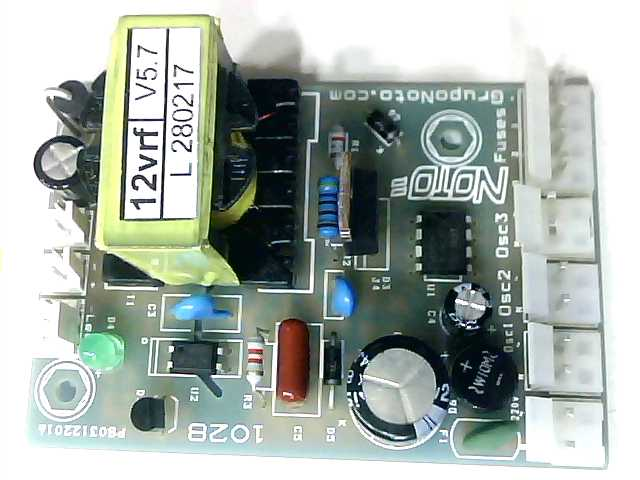
\includegraphics[width=0.24\textwidth]{./portfolio/fuente.jpg}
         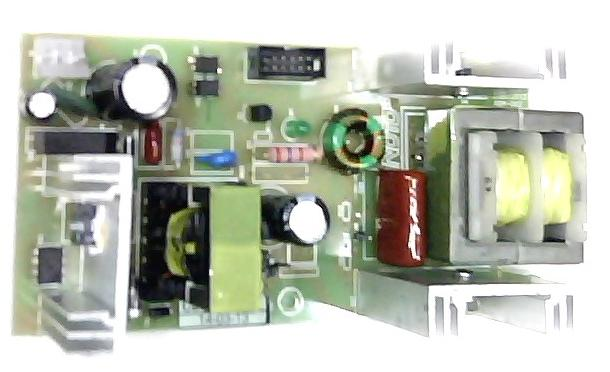
\includegraphics[width=0.24\textwidth]{./portfolio/cavi.jpeg}
         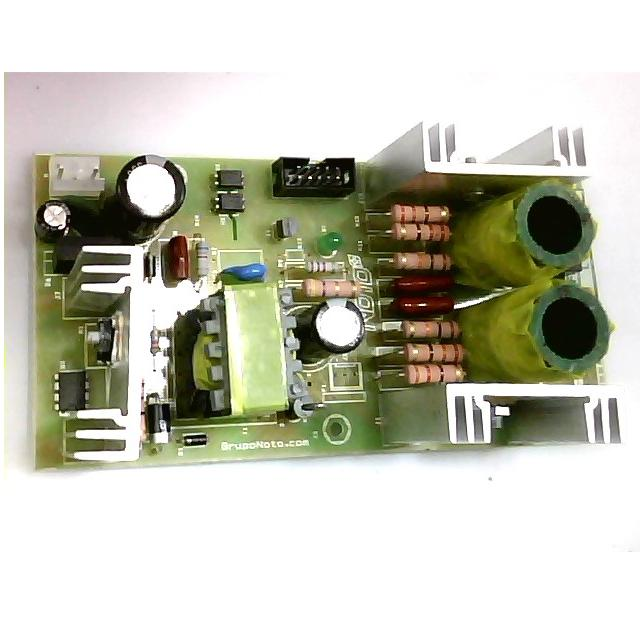
\includegraphics[width=0.24\textwidth]{./portfolio/trimax.jpeg}
         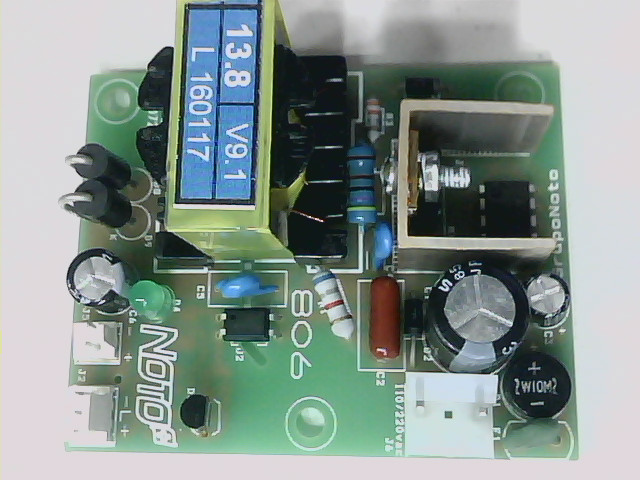
\includegraphics[width=0.24\textwidth]{./portfolio/fuente_13.jpeg}
      \end{center}
      \caption{Equipos de potencia, fuentes, osciladores, mezclando tecnologias TH y SMD}
      \label{fig:noto1}
   \end{figure}
   \begin{figure}
      \begin{center}
         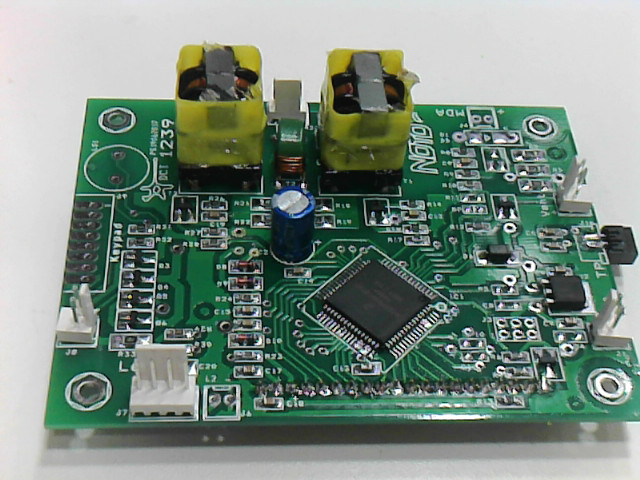
\includegraphics[width=0.24\textwidth]{./portfolio/n1500.png}
         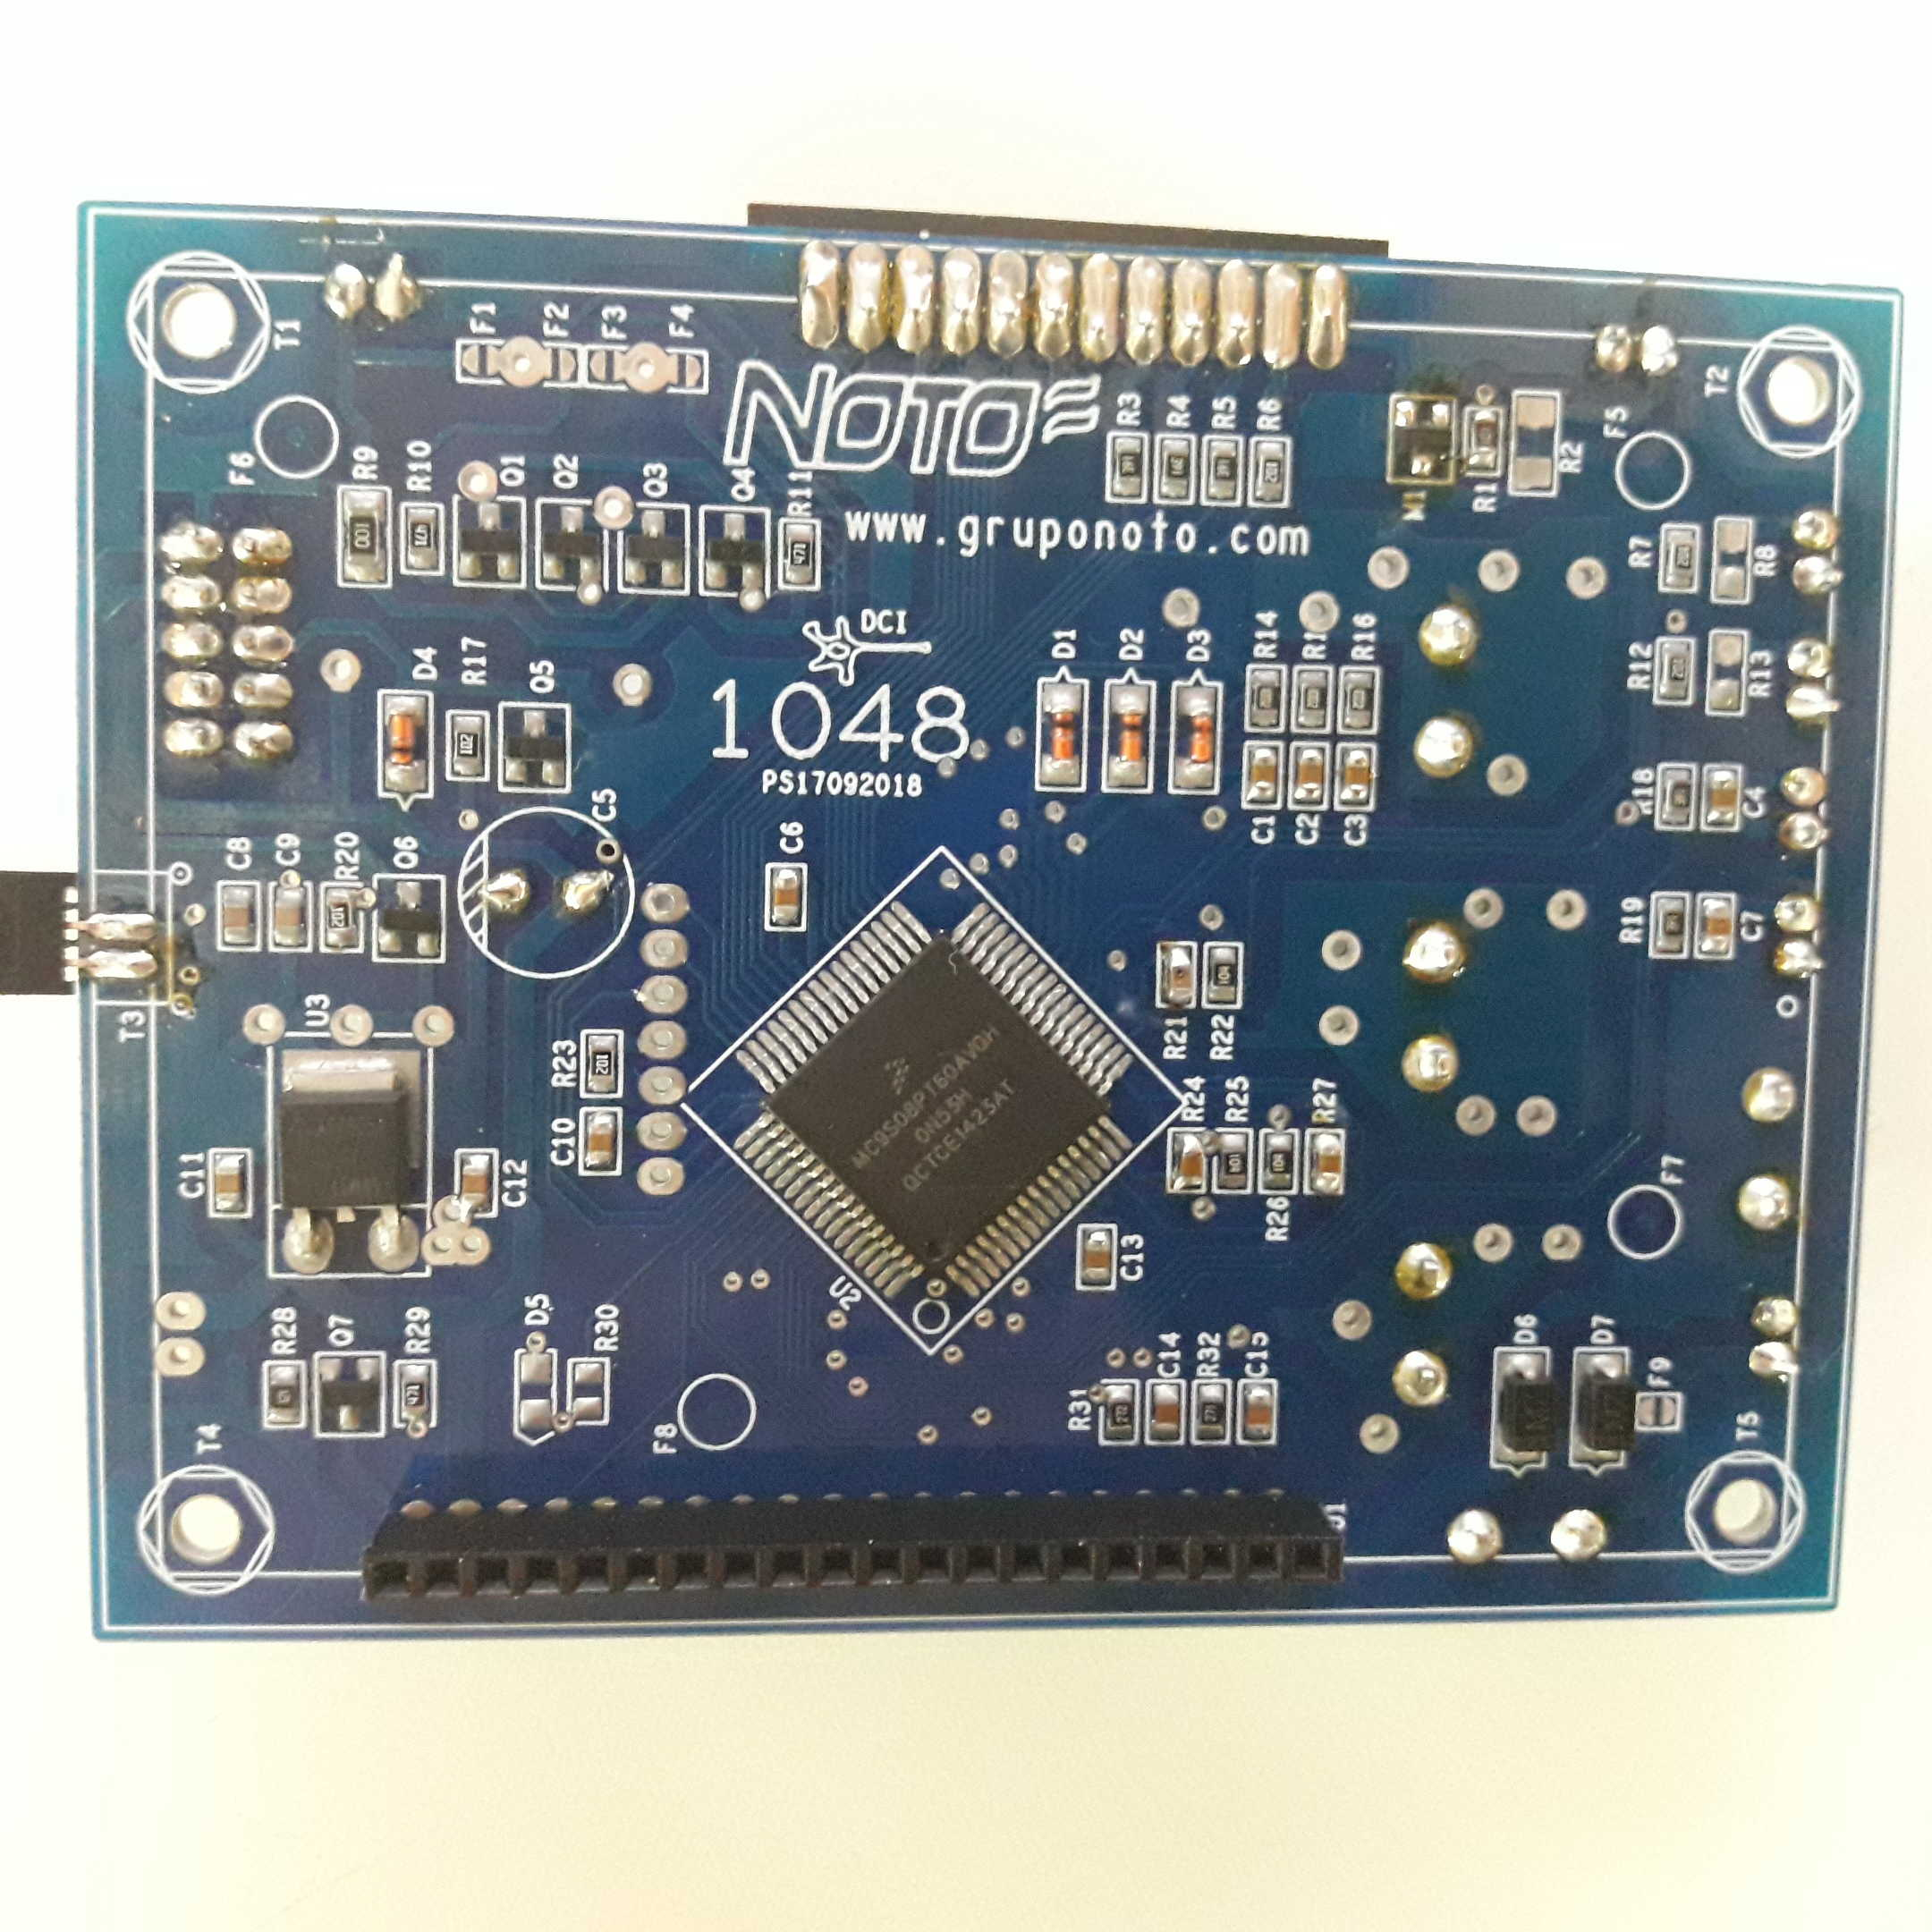
\includegraphics[width=0.24\textwidth]{./portfolio/lumiere.jpeg}
         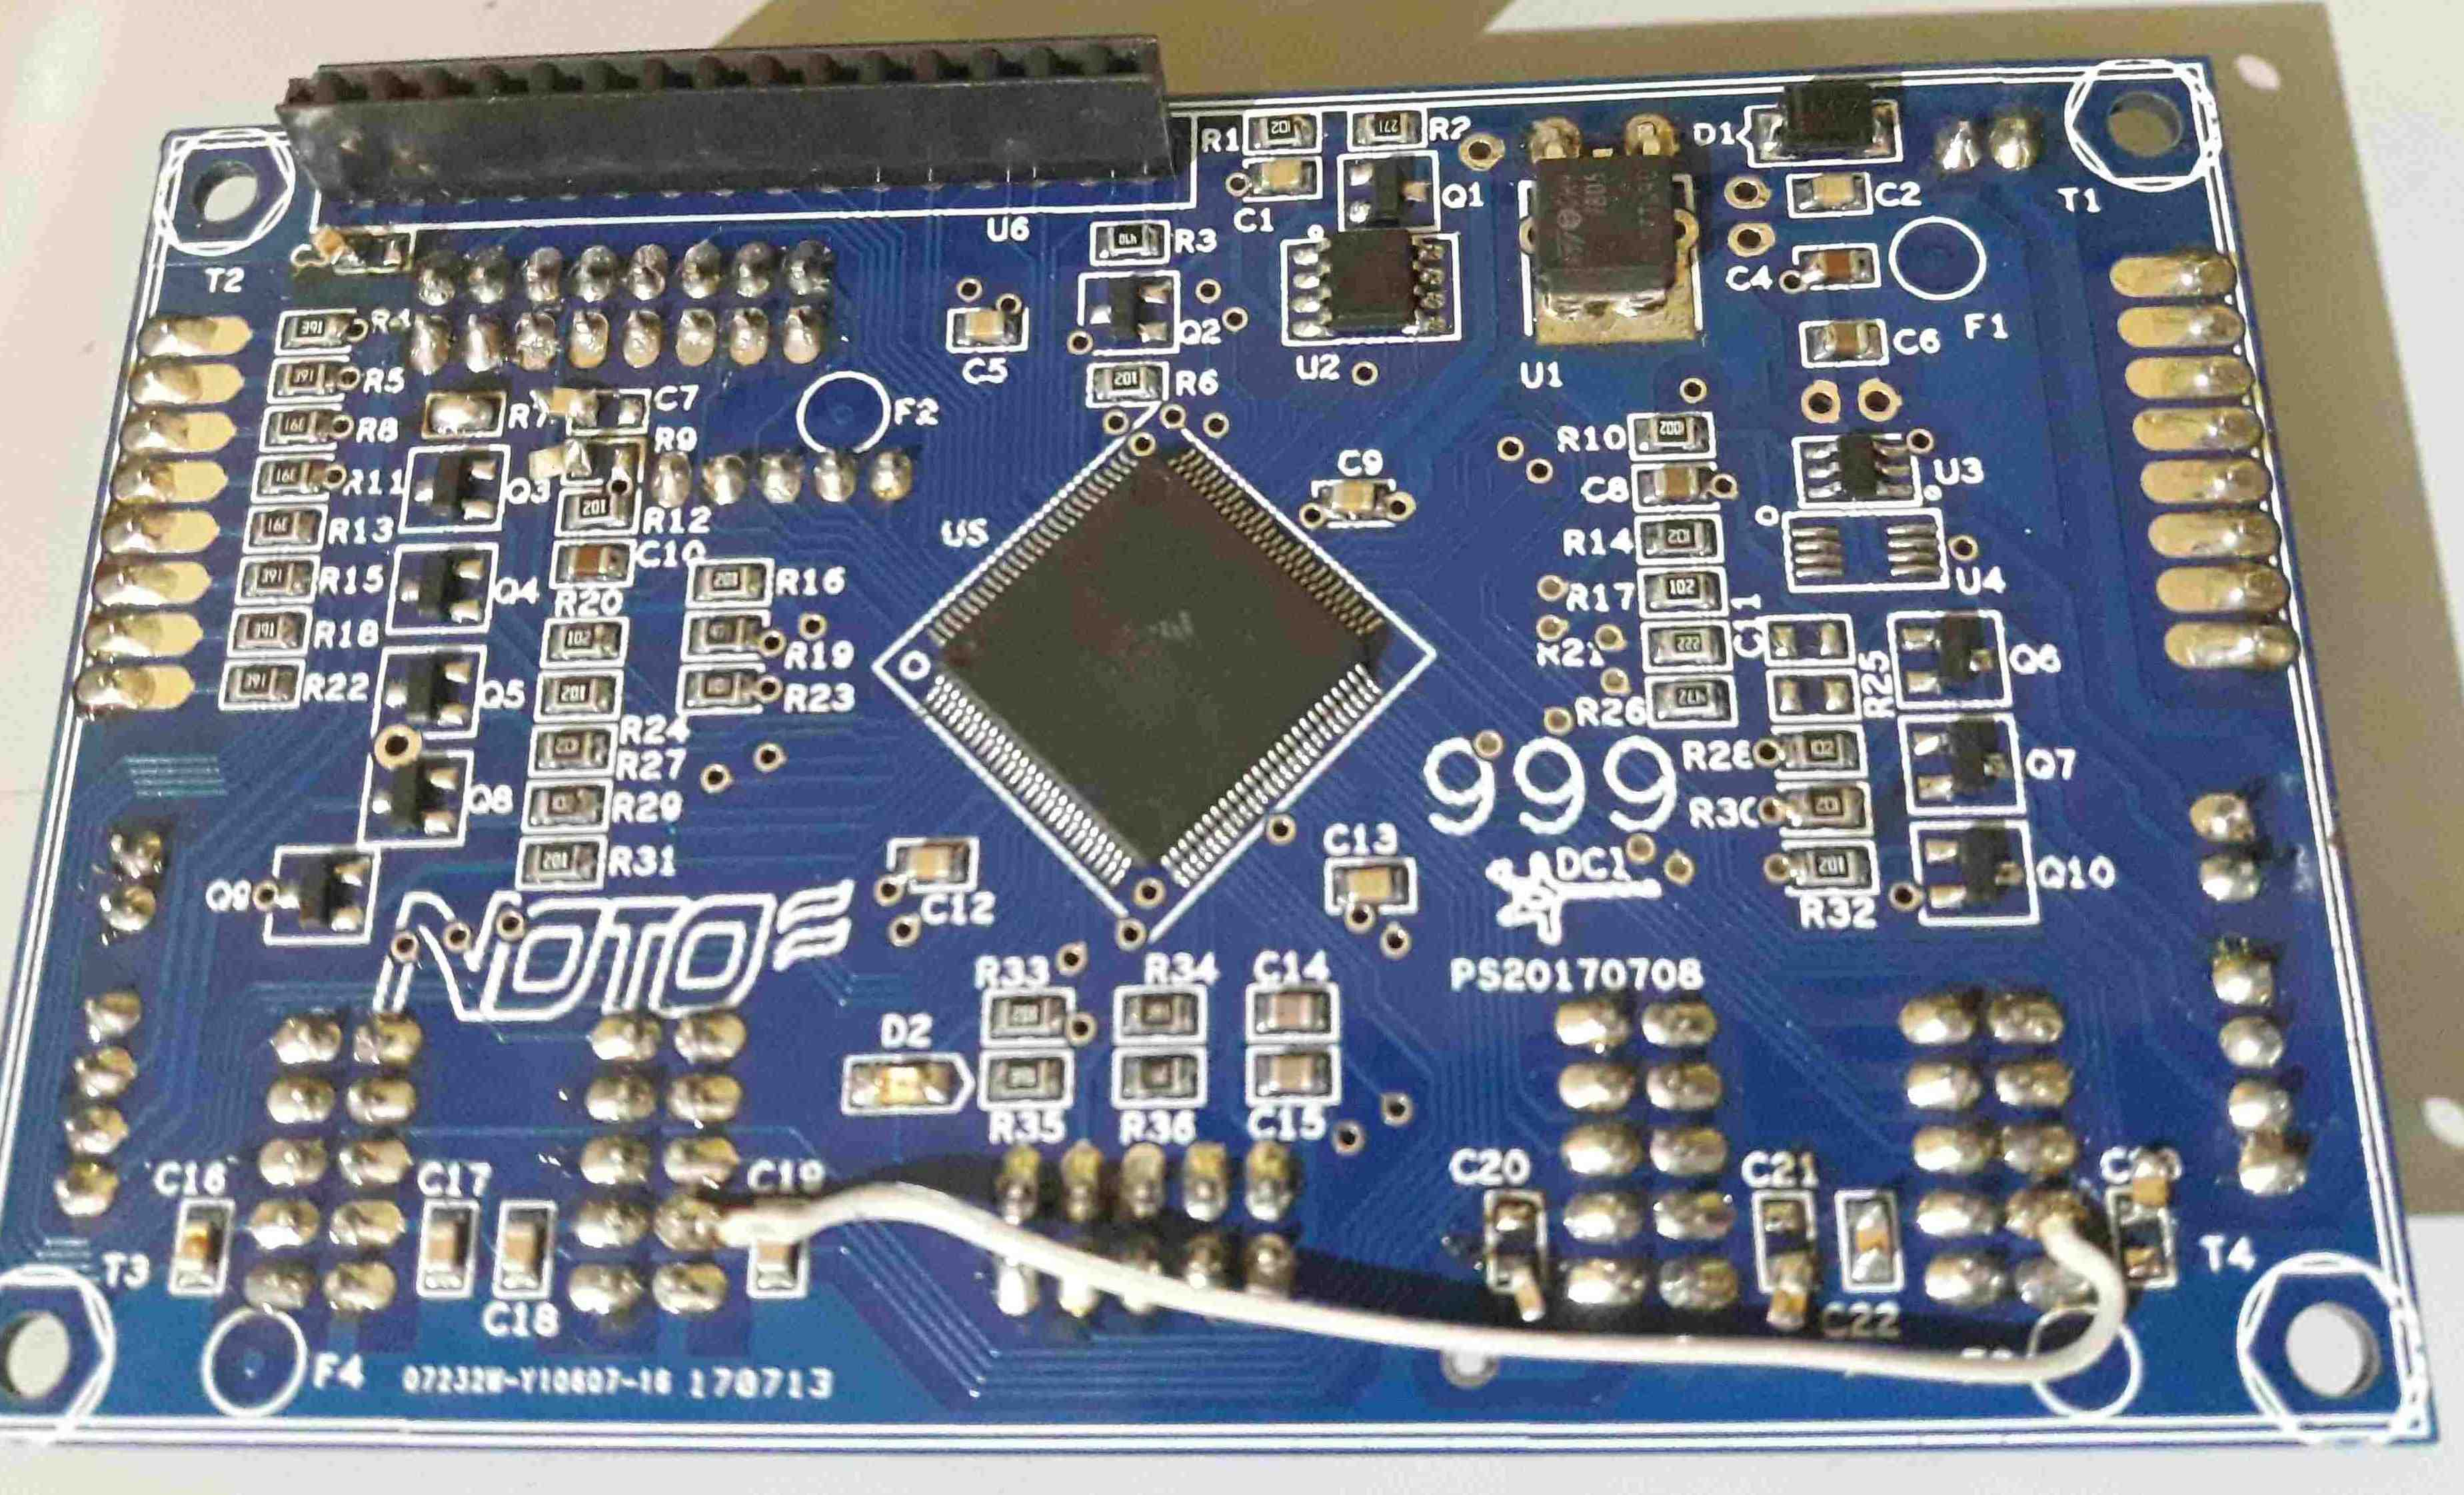
\includegraphics[width=0.24\textwidth]{./portfolio/electroestimulador.jpg}
         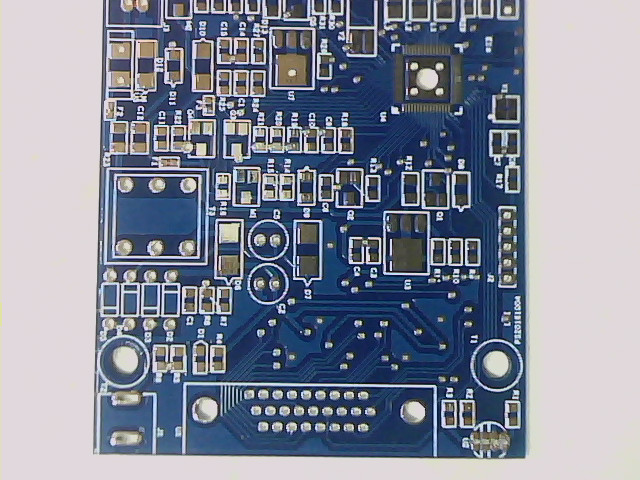
\includegraphics[width=0.24\textwidth]{./portfolio/electro_portatil_virgen.jpeg}
      \end{center}
      \caption{Placas de control para los diversos equipos, controladores de LCD, manejo de PWM, comunicaciones, generadores de señales, tecnología TH y SMD 1206, 0805 y 0603.}
      \label{fig:noto2}
   \end{figure}






